\documentclass{labreport}

\usepackage{microtype}
\usepackage{enumitem}
\usepackage{pifont}
\usepackage[T1]{fontenc}
\usepackage{amsmath,amssymb}
\usepackage{listings}
\usepackage{xcolor}
\usepackage{booktabs}
\usepackage{graphicx}
\usepackage{caption}
\usepackage{subcaption}
\usepackage{float}

% Colors matching os-lab1-2 style
\definecolor{codebg}{RGB}{248, 249, 251}
\definecolor{codeborder}{RGB}{218, 222, 229}
\definecolor{linkcolor}{RGB}{20, 60, 120}
\definecolor{zshgreen}{RGB}{0, 160, 80}
\definecolor{zshred}{RGB}{200, 30, 30}

% Hyperref setup with subtle link colors
\hypersetup{
    colorlinks=true,
    linkcolor=linkcolor,
    filecolor=linkcolor,
    urlcolor=linkcolor,
    citecolor=linkcolor
}

% Code and terminal listings
\lstdefinestyle{bash}{
    basicstyle=\ttfamily\footnotesize,
    backgroundcolor=\color{codebg},
    frame=single,
    framerule=0.5pt,
    rulecolor=\color{codeborder},
    breaklines=true,
    breakatwhitespace=false,
    showstringspaces=false,
    keepspaces=true,
    columns=flexible,
    numbers=none,
    xleftmargin=3pt,
    xrightmargin=3pt,
    framesep=4pt
}

\lstdefinestyle{python}{
    language=Python,
    basicstyle=\ttfamily\footnotesize,
    backgroundcolor=\color{codebg},
    frame=single,
    framerule=0.5pt,
    rulecolor=\color{codeborder},
    keywordstyle=\color{blue!85!black}\bfseries,
    commentstyle=\color{gray!80!black}\itshape,
    stringstyle=\color{teal!80!black},
    numbers=left,
    numberstyle=\tiny\color{gray!80!black},
    numbersep=8pt,
    breaklines=true,
    breakatwhitespace=false,
    showstringspaces=false,
    keepspaces=true,
    columns=flexible,
    tabsize=4,
    xleftmargin=14pt,
    xrightmargin=3pt,
    framesep=4pt
}

% Literate mappings for terminal glyphs and Romanian diacritics
\lstset{
    extendedchars=true,
    literate=
        {➜}{{\textcolor{zshgreen}{\ding{220}}}}{1}
        {├─}{|-\,}{2}
        {└─}{\`-\,}{2}
        {├}{|}{1}
        {─}{-}{1}
        {└}{\`}{1}
        {✗}{{\textcolor{zshred}{\ding{55}}}}{1}
        {Ă}{{\v{A}}}{1}
        {ă}{{\v{a}}}{1}
        {Â}{{\^A}}{1}
        {â}{{\^a}}{1}
        {Î}{{\^I}}{1}
        {î}{{\^i}}{1}
        {Ș}{{\cb{S}}}{1}
        {ș}{{\cb{s}}}{1}
        {Ț}{{\cb{T}}}{1}
        {ț}{{\cb{t}}}{1}
        {Ş}{{\cb{S}}}{1}
        {ş}{{\cb{s}}}{1}
        {Ţ}{{\cb{T}}}{1}
        {ţ}{{\cb{t}}}{1}
}

% Comma-below accent support for Romanian letters
\usepackage{combelow}

% Section styling for clean document structure
\titleformat{\section}
  {\large\bfseries}{\thesection}{0.8em}{}[\vspace{1pt}\hrule height 0.5pt]
\titleformat{\subsection}
  {\normalsize\bfseries}{\thesubsection}{0.8em}{}
\titleformat{\subsubsection}
  {\small\bfseries}{\thesubsubsection}{0.8em}{}

\begin{document}

\labtitle
    {1}
    {Caesar Cipher \& Caesar Cipher with Keyword Permutation}
    {st. gr. FAF-243}
    {Șoimu Ionuț}
    {asist. univ.\\[0.15cm] Zaica Maia}

\tableofcontents
\newpage

% ==============================================================================
\section{Introduction and Objectives}

Classical cryptography provides foundational principles for confidential communication. Among historical ciphers, monoalphabetic substitution ciphers represent the earliest attempts to obscure plaintext by systematically replacing characters according to fixed rules.

The objectives of this laboratory work are:
\begin{enumerate}[leftmargin=*]
    \item \textbf{Understand the mathematical foundations} and operational mechanics of the Caesar cipher.
    \item \textbf{Analyze the cryptographic weakness} of the Caesar cipher stemming from its trivial key space and vulnerability to brute-force attacks.
    \item \textbf{Implement keyword-based alphabet permutation} to significantly expand the key space and evaluate its effect on security.
    \item \textbf{Adapt classical algorithms to non-English alphabets}, specifically the 31-letter Romanian alphabet, enforcing strict indexing rules (Table 2) without relying on language-dependent ASCII/Unicode codepoint shifts.
    \item \textbf{Enforce robust input validation}, handling edge cases such as diacritic normalization (comma-below vs.\ cedilla), whitespace stripping, rejected character identification, and loop re-prompting.
\end{enumerate}

% ==============================================================================
\section{Short Theory}

\subsection{The Classical Caesar Cipher}

The Caesar cipher is an additive monoalphabetic substitution cipher attributed to Julius Caesar, who historically utilized a fixed shift of $k = 3$ to communicate military intelligence. Over an arbitrary finite alphabet $\Sigma$ of cardinality $n = |\Sigma|$, each symbol $m_i \in \Sigma$ is assigned a unique integer index $x_i \in \mathbb{Z}_n = \{0, 1, \dots, n-1\}$ through a bijective encoding function $\text{enc}: \Sigma \to \mathbb{Z}_n$.

The secret key $k$ is an integer chosen from the non-zero elements of the additive group $\mathbb{Z}_n$:
\begin{equation}
    k \in \mathcal{K} = \{1, 2, \dots, n-1\}.
\end{equation}
The identity key $k = 0$ is explicitly excluded since it maps every plaintext character directly to itself ($e_0(x) = x$), providing zero obfuscation.

\subsubsection{Encryption and Decryption Formulas}
For a plaintext message consisting of numeric codes $(x_1, x_2, \dots, x_N)$, encryption $e_k$ is computed using modular addition:
\begin{equation}
    c_i = e_k(x_i) = (x_i + k) \pmod n.
\end{equation}
Decryption $d_k$ is the inverse transformation under modular arithmetic, subtracting the secret key $k$:
\begin{equation}
    x_i = d_k(c_i) = (c_i - k) \pmod n.
\end{equation}
Because differences $(c_i - k)$ may produce negative integer values, the modulo operation must wrap around into the non-negative residue domain $[0, n-1]$:
\begin{equation}
    (c_i - k) \pmod n \equiv ((c_i - k) \bmod n + n) \bmod n.
\end{equation}

\subsubsection{Key Space and Security Vulnerabilities}
For the Romanian alphabet with $n = 31$, the key space is:
\begin{equation}
    |\mathcal{K}_{\text{Caesar}}| = n - 1 = 30.
\end{equation}
A key space of only 30 possible keys renders the cipher trivially vulnerable to an \textbf{exhaustive key search (brute-force attack)}. An adversary intercepting ciphertext $c$ can compute all 30 candidate plaintexts $d_1(c), d_2(c), \dots, d_{30}(c)$ instantaneously. Because natural language possesses high redundancy, exactly one candidate key yields readable Romanian text.

\subsection{The Caesar Cipher with a Permutation (Two Keys)}

To defend against trivial exhaustive search, the natural ordering of the alphabet can be permuted using a secondary secret key: a keyword $k_2$. The resulting cryptosystem utilizes two secret keys:
\begin{itemize}[noitemsep, topsep=2pt]
    \item \textbf{Key 1 ($k_1$):} The numeric Caesar shift value, $k_1 \in \{1, 2, \dots, n-1\}$.
    \item \textbf{Key 2 ($k_2$):} A keyword string consisting of Romanian letters with length $|k_2| \ge 7$.
\end{itemize}

\subsubsection{Permuted Alphabet Construction}
The permuted alphabet $\Sigma_{\text{perm}} = (\sigma'_0, \sigma'_1, \dots, \sigma'_{n-1})$ is assembled deterministically:
\begin{enumerate}[leftmargin=*]
    \item Convert $k_2$ to uppercase and filter out spaces or diacritic variations.
    \item Extract the distinct letters of $k_2$ in their order of initial appearance, discarding duplicate occurrences.
    \item Append the remaining letters of the original alphabet $\Sigma$ that were not in $k_2$, preserving their original canonical ordering (Table 2).
\end{enumerate}

\subsubsection{Encryption and Decryption over the Permuted Domain}
Let $\text{pos}_{\text{perm}}(s)$ denote the index of character $s$ within $\Sigma_{\text{perm}}$. The cryptographic transformations are defined as:
\begin{equation}
    c_i = \Sigma_{\text{perm}}\left[ (\text{pos}_{\text{perm}}(m_i) + k_1) \pmod n \right],
\end{equation}
\begin{equation}
    m_i = \Sigma_{\text{perm}}\left[ (\text{pos}_{\text{perm}}(c_i) - k_1) \pmod n \right].
\end{equation}

\subsubsection{Key Space Analysis and Cryptanalytic Resilience}
The number of distinct permutations of an $n$-element alphabet is given by the factorial $n!$. For $n = 31$:
\begin{equation}
    31! \approx 8.2228 \times 10^{33}.
\end{equation}
Combined with the 30 possible shifts of $k_1$, the theoretical key pair space is:
\begin{equation}
    |\mathcal{K}_{\text{total}}| = 30 \times 31! \approx 2.4668 \times 10^{35}.
\end{equation}
While keyword-derived permutations span a subset of all $31!$ permutations (due to dictionary word constraints), the effective search space far exceeds $10^{15}$ candidates, entirely neutralizing brute-force enumeration.

However, \textbf{the cipher remains a monoalphabetic substitution cipher}. A fixed plaintext character $x$ is mapped to the exact same ciphertext character $c$ throughout the entire message. Therefore:
\begin{itemize}[noitemsep, topsep=2pt]
    \item The unigram, bigram, and trigram frequency distributions of the source language are fully preserved in the ciphertext.
    \item In Romanian, vowels (\texttt{E}, \texttt{I}, \texttt{A}) and consonants (\texttt{R}, \texttt{T}, \texttt{N}) occur with distinct probability peaks.
    \item A cryptanalyst can bypass the keyword and shift entirely by performing \textbf{frequency analysis}, matching high-frequency ciphertext symbols to known Romanian language statistics.
\end{itemize}

% ==============================================================================
\section{Implementation Details}

\subsection{Architecture and Romanian Alphabet Representation}

The implementation was constructed in Python with a clean, modular architecture separated into distinct components:
\begin{itemize}[noitemsep, topsep=2pt]
    \item \texttt{romanian\_alphabet.py}: Canonical definition of Table 2, diacritic normalizers, permutation builders, and validation routines.
    \item \texttt{caesar\_cipher.py}: Task 1.1 single-key Caesar cipher implementation with interactive user prompts and re-prompting loops.
    \item \texttt{caesar\_permuted.py}: Task 1.2 two-key Caesar cipher implementation with permuted alphabet generation and inspection table formatting.
    \item \texttt{main.py}: Unified CLI and interactive interface supporting parameter parsing, automated demonstrations, and user workflows.
\end{itemize}

Table~\ref{tab:romanian_alphabet} outlines the canonical Table 2 encoding prescribed by the laboratory specifications for $n = 31$.

\begin{table}[H]
\centering
\small
\caption{Canonical Romanian Alphabet Letter Encoding ($n = 31$, Table 2)}
\label{tab:romanian_alphabet}
\begin{tabular}{@{}l*{16}{c}@{}}
\toprule
\textbf{Letter} & A & Ă & Â & B & C & D & E & F & G & H & I & Î & J & K & L & M \\
\textbf{Code}   & 0 & 1 & 2 & 3 & 4 & 5 & 6 & 7 & 8 & 9 & 10 & 11 & 12 & 13 & 14 & 15 \\
\midrule
\textbf{Letter} & N & O & P & Q & R & S & Ș & T & Ț & U & V & W & X & Y & Z & -- \\
\textbf{Code}   & 16 & 17 & 18 & 19 & 20 & 21 & 22 & 23 & 24 & 25 & 26 & 27 & 28 & 29 & 30 & -- \\
\bottomrule
\end{tabular}
\end{table}

\subsection{Code Fragments and Explanations}

\subsubsection{Alphabet Definition and Explicit Mapping}
The lab strictly requires that built-in ASCII/Unicode code point arithmetic must not be used to compute the Caesar shift. Instead, an explicit list and bidirectional dictionary mappings are established:

\begin{lstlisting}[style=python]
ROMANIAN_ALPHABET: List[str] = [
    'A', 'Ă', 'Â', 'B', 'C', 'D', 'E', 'F', 'G', 'H', 'I',
    'Î', 'J', 'K', 'L', 'M', 'N', 'O', 'P', 'Q', 'R', 'S',
    'Ș', 'T', 'Ț', 'U', 'V', 'W', 'X', 'Y', 'Z'
]
ALPHABET_SIZE: int = len(ROMANIAN_ALPHABET)  # 31

CHAR_TO_INDEX: Dict[str, int] = {char: idx for idx, char in enumerate(ROMANIAN_ALPHABET)}
INDEX_TO_CHAR: Dict[int, str] = {idx: char for idx, char in enumerate(ROMANIAN_ALPHABET)}
\end{lstlisting}
\textbf{Comment:} This defines the exact domain $\mathbb{Z}_{31}$. Mapping lookup is $O(1)$ and guarantees that letter substitutions strictly follow Table 2 rather than ASCII offsets.

\subsubsection{Diacritic Normalization and Cedilla Compatibility}
Romanian keyboards and typography frequently interchange comma-below letters (\texttt{Ș}, \texttt{Ț} -- Unicode \texttt{U+0218}, \texttt{U+021A}) with Turkish-style cedilla variants (\texttt{Ş}, \texttt{Ţ} -- Unicode \texttt{U+015E}, \texttt{U+0162}). To ensure compatibility across different operating systems and keyboards, an explicit normalizer was implemented:

\begin{lstlisting}[style=python]
CEDILLA_MAPPING: Dict[str, str] = {
    'Ş': 'Ș', 'ş': 'ș',
    'Ţ': 'Ț', 'ţ': 'ț',
}

def normalize_text(text: str) -> str:
    """Normalizes cedillas to comma-below and converts to uppercase."""
    normalized_chars = [CEDILLA_MAPPING.get(c, c).upper() for c in text]
    return "".join(normalized_chars)
\end{lstlisting}
\textbf{Comment:} All input characters are converted to standard comma-below representations before any membership validation or cryptographic transformation occurs.

\subsubsection{Strict Input Validation and Error Reporting}
The laboratory specification requires rejecting invalid keys or non-alphabet characters with a clear message indicating the allowed range and the exact rejected character.

\begin{lstlisting}[style=python]
def validate_key(key_input: str) -> Tuple[bool, Optional[str], int]:
    try:
        k = int(key_input.strip())
    except ValueError:
        return False, f"Error: Invalid key '{key_input}'. Must be integer 1..30.", -1
    if 1 <= k <= (ALPHABET_SIZE - 1):
        return True, None, k
    return False, f"Error: Key {k} out of range. Allowed: 1..30 inclusive.", -1

def validate_text(raw_text: str) -> Tuple[bool, Optional[str], str]:
    if not raw_text:
        return False, "Error: Text input cannot be empty.", ""
    normalized = normalize_text(raw_text)
    cleaned_chars = []
    for idx, ch in enumerate(normalized):
        if ch.isspace():
            continue
        if ch in CHAR_TO_INDEX:
            cleaned_chars.append(ch)
        else:
            orig = raw_text[idx]
            return False, (
                f"Error: Invalid character '{orig}' (U+{ord(orig):04X}) at pos {idx + 1}.\n"
                f"Allowed characters: Romanian alphabet letters (A-Z, Ă, Â, Î, Ș, Ț) and spaces."
            ), ""
    return True, None, "".join(cleaned_chars)
\end{lstlisting}
\textbf{Comment:} Spaces are permitted in user input and stripped automatically. Any foreign symbol (numbers, punctuation, symbols) is caught immediately, highlighting the 1-indexed character position and its Unicode codepoint.

\subsubsection{Building the Permuted Alphabet}
For Task 1.2, the permuted alphabet is constructed by deduplicating the keyword and appending the remaining Romanian letters:

\begin{lstlisting}[style=python]
def build_permuted_alphabet(keyword: str) -> List[str]:
    normalized_kw = normalize_text(keyword)
    permuted: List[str] = []
    seen = set()

    for ch in normalized_kw:
        if ch in CHAR_TO_INDEX and ch not in seen:
            seen.add(ch)
            permuted.append(ch)

    for ch in ROMANIAN_ALPHABET:
        if ch not in seen:
            seen.add(ch)
            permuted.append(ch)

    assert len(permuted) == ALPHABET_SIZE
    return permuted
\end{lstlisting}
\textbf{Comment:} Preserves the insertion order of unique keyword characters, guarantees that all 31 Romanian alphabet symbols are present exactly once, and maintains a linear $O(n)$ complexity.

\subsubsection{Encryption and Decryption Algorithms}
Both Task 1.1 and Task 1.2 transformations map characters to indices, apply modular shifts, and map indices back to the corresponding alphabet:

\begin{lstlisting}[style=python]
def encrypt_caesar(plaintext: str, key: int) -> str:
    return "".join(INDEX_TO_CHAR[(CHAR_TO_INDEX[c] + key) % ALPHABET_SIZE] for c in plaintext)

def decrypt_caesar(ciphertext: str, key: int) -> str:
    return "".join(INDEX_TO_CHAR[(CHAR_TO_INDEX[c] - key) % ALPHABET_SIZE] for c in ciphertext)

def encrypt_caesar_permuted(plaintext: str, key1: int, permuted: List[str]) -> str:
    char_to_pos = {char: idx for idx, char in enumerate(permuted)}
    return "".join(permuted[(char_to_pos[c] + key1) % ALPHABET_SIZE] for c in plaintext)

def decrypt_caesar_permuted(ciphertext: str, key1: int, permuted: List[str]) -> str:
    char_to_pos = {char: idx for idx, char in enumerate(permuted)}
    return "".join(permuted[(char_to_pos[c] - key1) % ALPHABET_SIZE] for c in ciphertext)
\end{lstlisting}
\textbf{Comment:} Python's native modulo operator \texttt{\%} implements mathematical floored division, ensuring that \texttt{(y - key) \% 31} always produces a positive residue in the range $[0, 30]$.

% ==============================================================================
\section{Results and Demonstration}

\subsection{Task 1.1: Single-Key Caesar Cipher Execution}

\subsubsection{Operational Verification and Hand Calculation}
Consider encrypting the Romanian test string:
\begin{center}
    \texttt{"Cifrul Cezar cu caractere românești"}
\end{center}
with shift key $k = 5$.
\begin{enumerate}[leftmargin=*]
    \item \textbf{Preprocessing:} Spaces are stripped, cedillas converted, and text cast to uppercase:
    \begin{center}
        \texttt{"CIFRULCEZARCUCARACTEREROMÂNEȘTI"}
    \end{center}
    \item \textbf{Letter Transformation Steps (Excerpt):}
    \begin{itemize}[noitemsep, topsep=2pt]
        \item \texttt{C}: Code $4 \implies (4 + 5) \bmod 31 = 9 \implies \texttt{H}$
        \item \texttt{I}: Code $10 \implies (10 + 5) \bmod 31 = 15 \implies \texttt{M}$
        \item \texttt{F}: Code $7 \implies (7 + 5) \bmod 31 = 12 \implies \texttt{J}$
        \item \texttt{R}: Code $20 \implies (20 + 5) \bmod 31 = 25 \implies \texttt{U}$
        \item \texttt{U}: Code $25 \implies (25 + 5) \bmod 31 = 30 \implies \texttt{Z}$
        \item \texttt{L}: Code $14 \implies (14 + 5) \bmod 31 = 19 \implies \texttt{Q}$
        \item \texttt{Z}: Code $30 \implies (30 + 5) \bmod 31 = 4 \implies \texttt{C}$ (Wrap-around)
        \item \texttt{Ș}: Code $22 \implies (22 + 5) \bmod 31 = 27 \implies \texttt{W}$
        \item \texttt{Ț}: Code $24 \implies (24 + 5) \bmod 31 = 29 \implies \texttt{Y}$
    \end{itemize}
    \item \textbf{Ciphertext Produced:} \texttt{"HMJUZQHÎCDUHZHDUDHXÎUÎUȘRFSÎ"}
    \item \textbf{Decryption Verification:} Applying the decryption function $d_5(y) = (y - 5) \bmod 31$ to each character of the ciphertext restores the identical original plaintext string.
\end{enumerate}

Figure~\ref{fig:task1_valid} illustrates the terminal session in the Kitty terminal running \texttt{caesar\_cipher.py}, displaying the canonical Romanian alphabet mapping table, successful encryption of the phrase, and reciprocal decryption verifying round-trip correctness.

\begin{figure}[H]
    \centering
    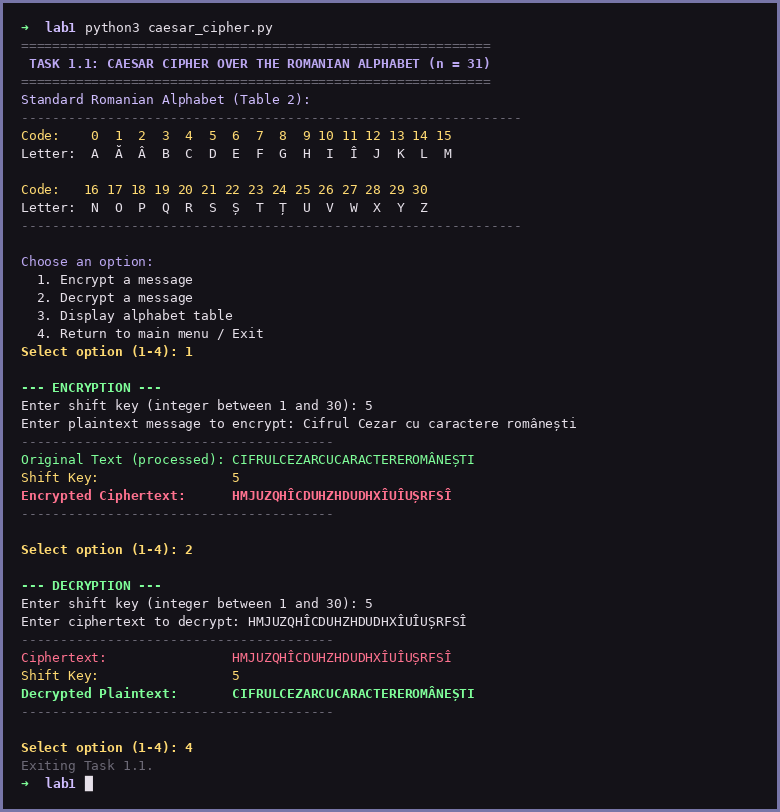
\includegraphics[width=0.88\linewidth]{figures/screenshot_task1_valid.png}
    \caption{Task 1.1 terminal capture: Encryption and decryption execution over Romanian alphabet with diacritics.}
    \label{fig:task1_valid}
\end{figure}

\subsection{Task 1.1: Error Handling and Input Validation}

The implementation strictly validates user input and displays informative error diagnostics before requesting the value again:
\begin{itemize}[noitemsep, topsep=2pt]
    \item \textbf{Out-of-range Shift Key:} Inputting $k = 35$ produces a message stating the allowed interval $1 \le k \le 30$.
    \item \textbf{Non-numeric Key:} Entering non-integer string values such as \texttt{"abc"} is caught and rejected gracefully.
    \item \textbf{Illegal Characters:} Entering \texttt{"Salut 2026!"} isolates character \texttt{'2'} at position 7 as non-Romanian and displays the allowed alphabet range before re-prompting.
    \item \textbf{Recovery:} Valid text \texttt{"Securitate Informațională"} with key $k = 7$ is successfully processed into \texttt{"YJFÂYNĂĂGNPUTVRĂȚNTUTĂF"}.
\end{itemize}

Figure~\ref{fig:task1_errors} documents this validation behavior and prompt recovery sequence in the terminal.

\begin{figure}[H]
    \centering
    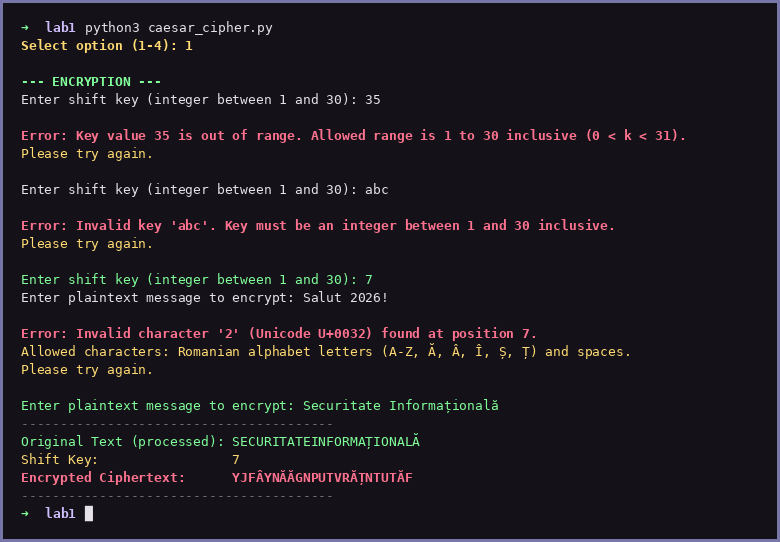
\includegraphics[width=0.88\linewidth]{figures/screenshot_task1_errors.png}
    \caption{Task 1.1 terminal capture: Diagnostic messages for out-of-range keys, non-numeric inputs, and illegal character positions.}
    \label{fig:task1_errors}
\end{figure}

\subsection{Task 1.2: Two-Key Caesar Cipher with Permutation}

\subsubsection{Permuted Alphabet Generation and Hand-Check Verification}
Using keyword $k_2 = \texttt{"CRIPTOGRAFIE"}$ ($|k_2| = 12 \ge 7$):
\begin{enumerate}[leftmargin=*]
    \item \textbf{Unique Keyword Characters:} \texttt{C, R, I, P, T, O, G, A, F, E} (subsequent occurrences of \texttt{R} and \texttt{I} are discarded).
    \item \textbf{Remaining Letters Appended:} Ă, Â, B, D, H, Î, J, K, L, M, N, Q, S, Ș, Ț, U, V, W, X, Y, Z.
    \item \textbf{Resulting Permuted Alphabet (Table~\ref{tab:permuted_table}):}
\end{enumerate}

\begin{table}[H]
\centering
\small
\caption{Permuted Romanian Alphabet for Keyword \texttt{"CRIPTOGRAFIE"}}
\label{tab:permuted_table}
\begin{tabular}{@{}l*{16}{c}@{}}
\toprule
\textbf{Pos}    & 0 & 1 & 2 & 3 & 4 & 5 & 6 & 7 & 8 & 9 & 10 & 11 & 12 & 13 & 14 & 15 \\
\textbf{Letter} & C & R & I & P & T & O & G & A & F & E & Ă & Â & B & D & H & Î \\
\midrule
\textbf{Pos}    & 16 & 17 & 18 & 19 & 20 & 21 & 22 & 23 & 24 & 25 & 26 & 27 & 28 & 29 & 30 & -- \\
\textbf{Letter} & J & K & L & M & N & Q & S & Ș & Ț & U & V & W & X & Y & Z & -- \\
\bottomrule
\end{tabular}
\end{table}

Encrypting \texttt{"CALCULATOARE SI MICROELECTRONICA"} with shift $k_1 = 3$:
\begin{itemize}[noitemsep, topsep=2pt]
    \item \texttt{C}: Pos $0 \implies (0 + 3) \bmod 31 = 3 \implies \texttt{P}$
    \item \texttt{A}: Pos $7 \implies (7 + 3) \bmod 31 = 10 \implies \texttt{Ă}$
    \item \texttt{L}: Pos $18 \implies (18 + 3) \bmod 31 = 21 \implies \texttt{Q}$
    \item \texttt{C}: Pos $0 \implies 3 \implies \texttt{P}$
    \item \texttt{U}: Pos $25 \implies (25 + 3) \bmod 31 = 28 \implies \texttt{X}$
\end{itemize}
Yielding the ciphertext: \texttt{"PĂQPXQĂAFĂTBUOSOPTFBQBPATFȘOPĂ"}.

Figure~\ref{fig:task2_valid} demonstrates the execution of \texttt{caesar\_permuted.py}, displaying the permuted alphabet for manual verification followed by two-key encryption and decryption.

\begin{figure}[H]
    \centering
    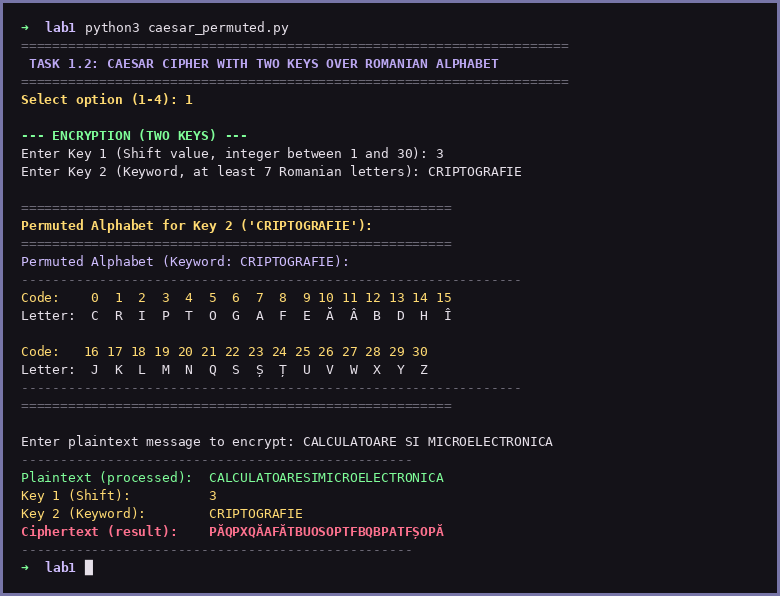
\includegraphics[width=0.88\linewidth]{figures/screenshot_task2_valid.png}
    \caption{Task 1.2 terminal capture: Permuted alphabet displayed for verification, followed by two-key encryption and decryption.}
    \label{fig:task2_valid}
\end{figure}

\subsection{Task 1.2: Error Handling for Keyword and Shift Keys}

Figure~\ref{fig:task2_errors} captures the error handling for Task 1.2 inputs:
\begin{itemize}[noitemsep, topsep=2pt]
    \item \textbf{Shift Boundary Enforcement:} Key $k_1 = 0$ is rejected with a range notice ($1 \le k_1 \le 30$).
    \item \textbf{Keyword Length Threshold:} Keyword \texttt{"CEZAR"} (length 5) is rejected because the task requires $|k_2| \ge 7$.
    \item \textbf{Keyword Character Validation:} Keyword \texttt{"CRIPTO\#SEC"} is rejected due to illegal character \texttt{'\#'} at position 7.
    \item \textbf{Recovery:} A valid keyword \texttt{"SECRETLAB"} is accepted, and its permuted alphabet is printed.
\end{itemize}

\begin{figure}[H]
    \centering
    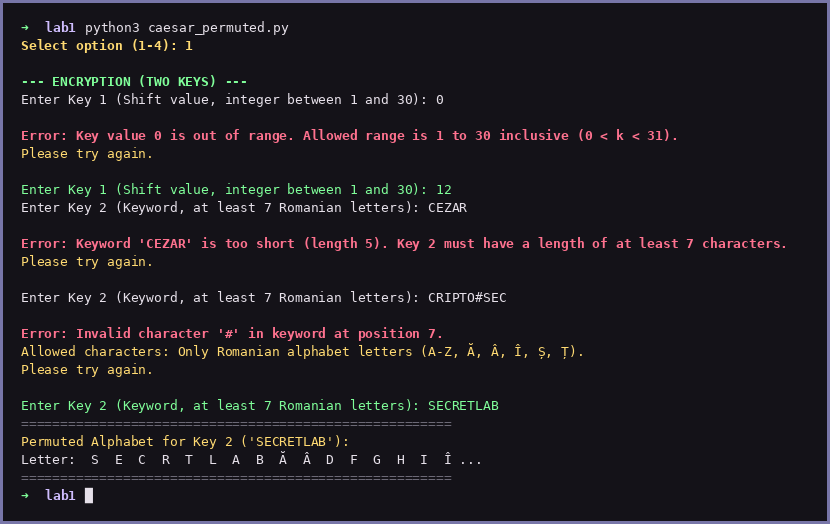
\includegraphics[width=0.88\linewidth]{figures/screenshot_task2_errors.png}
    \caption{Task 1.2 terminal capture: Validation errors for shift bounds, short keywords, and illegal symbols.}
    \label{fig:task2_errors}
\end{figure}

\newpage
% ==============================================================================
\section{Conclusions}
\markboth{5\quad Conclusions}{5\quad Conclusions}

Through this laboratory work, I implemented and evaluated two classical substitution ciphers adapted to the Romanian language: the standard single-key Caesar cipher and the keyword-permuted two-key Caesar cipher.

\begin{itemize}[leftmargin=*]
    \item \textbf{Key Space and Brute-Force Resilience:} The standard Caesar cipher over the 31-letter Romanian alphabet possesses only 30 possible keys, making exhaustive search trivial by hand or on a computer. In contrast, introducing a keyword permutation expands the theoretical permutation space to $31! \times 30 \approx 2.47 \times 10^{35}$, completely eliminating brute-force search as a viable attack vector.
    \item \textbf{Vulnerability to Frequency Analysis:} Despite the massive expansion in key space, the two-key Caesar cipher remains a monoalphabetic substitution cipher. Because the mapping from plaintext to ciphertext letters is 1-to-1 and stationary, language statistics (such as the high frequency of Romanian letters \texttt{E}, \texttt{I}, \texttt{A}, \texttt{R}, and \texttt{T}) remain intact in the ciphertext. Thus, an attacker armed with ciphertext of sufficient length can recover the plaintext using frequency analysis without discovering the secret keyword.
    \item \textbf{Alphabet Handling and Engineering Considerations:} Restricting the cipher to Table 2 required avoiding ASCII/Unicode arithmetic shortcuts and implementing custom index lookups. Handling Romanian diacritics also required normalising cedilla characters (\texttt{Ş}, \texttt{Ţ}) to standard comma-below characters (\texttt{Ș}, \texttt{Ț}).
\end{itemize}

In conclusion, this work demonstrated that expanding key space alone does not ensure cryptographic security if structural statistical patterns are preserved. Truly secure symmetric encryption requires diffusion and confusion principles (as found in polyalphabetic ciphers and modern block ciphers like AES).

% ==============================================================================
\section{Source Code Repository}
\markboth{5\quad Conclusions}{5\quad Conclusions}

The complete source code and report build files are organized in the project repository:

\begin{center}
    \textbf{GitHub Repository Link:}\\
    \url{https://github.com/USER/REPO-PLACEHOLDER}
\end{center}

\end{document}
